%! Author = smen851
%! Date = 19/08/2023

% Preamble
\documentclass[11pt,a4paper]{article}

% Packages
\usepackage{amsmath}
\usepackage{import} % for latex pdf figs
\usepackage{graphicx}
\usepackage{color}
\usepackage{amsfonts}
\usepackage{subfig}
\usepackage[utf8]{inputenc}
\usepackage{hyperref}
\usepackage[shortlabels]{enumitem}
\usepackage{drftcite}
% MACROS
% referencing a section
\newcommand{\sref}[1]{Section~\ref{#1}}
% referencing a figure
\newcommand{\fig}[1]{Fig.~\ref{#1}}
% referencing a table
\newcommand{\tabl}[1]{Table~\ref{#1}}
% quoting (ref: https://www.youtube.com/watch?v=voSpOrimkMY&ab )
\newcommand{\laser}[1]{``#1''}
% sinc
\DeclareMathOperator{\sinc}{sinc}
\graphicspath{ {./figures/} }

% title settings
\title{Microstrip Line Test and Results}
\author{Simone Mencarelli}

% Document
\begin{document}
    % title
    \maketitle


    \section{Relevant documents}
    \label{sec:relevant-documents}
    \begin{enumerate}[start=1,label={[Doc\arabic*]}]
        \item S.M., \laser{\emph{Microstrip Line Characterization}}, August 2023 \label{doc:microstrip-characterization}
    \end{enumerate}


    \section{Introduction}
    \label{sec:introduction}
    \begin{figure}[!h]
        \includegraphics[width=\textwidth]{fixture}
        \caption{Smaller 40~mm line test fixture. Front: 5~mm~x~40~mm adhesive copper trace on glass fiber slab.
        Back: thru-hole SMA connector with m2.5 screws and bolts.}
        \label{fig:photo}
    \end{figure}
    This report contains the results for the microstrip line test produced using vector measurements of the reflection
    and transmission frequency response of three test fixtures of different lengths.
    The shorter fixture is shown in \fig{fig:photo}.
    The three fixtures feature a microstrip line built using an adhesive copper strip 5~mm wide on a piece of dielectric
    composite (Material Under Test) glued on a supporting aluminium slab.
    Two thru-hole connectors are bolted to the structure with the central pin trimmed to length and soldered to the copper line.
    From here on, the fixtures are referred to by their line length; respectively: long~=~219~mm (L), medimum~=~146~mm (M), and
    short~=~40mm (S).\\
    The complex propagation coefficient $\gamma$ extraction procedure is defined in \ref{doc:microstrip-characterization} and
    applied here with minor modifications.
    An overview of the methodology and the results of this de-embedding procedure are reported in~\sref{sec:de-embedding}.\\
    The error sensitivity to small differences in the average permittivity of the fixtures is derived in~\sref{sec:error}
    in an effort to explain the discrepancies found in the results of~\sref{sec:de-embedding}.\\
    The procedure for fitting the measured datum to a CST microstrip model is reported in~\sref{sec:numerical-model-matching}
    along with the resulting permittivity and loss tangent of the \emph{Material Under Test} (MUT).\\
    The conclusions are drawn~\sref{sec:conclusion}.


    \section{Fixtures assembly and geometrical variability}
    \label{sec:assembly}


    \section{De-embedding results}
    \label{sec:de-embedding}

    \subsection{Simulated data reference}
    \label{subsec:simulation}
    \begin{figure}[!h]
        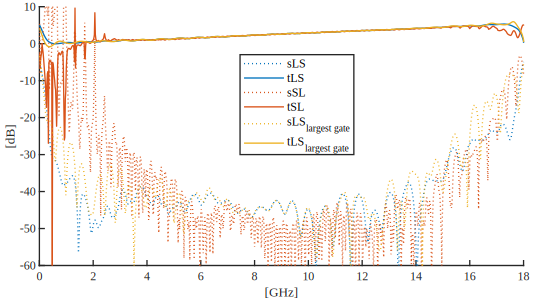
\includegraphics[width=\textwidth]{sparasim}
        \caption{De-embedding results from full wave simulations of a 40~mm (S) and a 219~mm (L) test fixtures.
        Solid lines: transmissivity (s), dotted lines: reflectivity (t); for all the combinations plus LS deembedding
        without gate width variation. The transmissivity sign is chosen to always correspond to a negative-length section
        of lossy transmission line (for ease of comparison).}
        \label{fig:sparasim}
    \end{figure}
    \begin{figure}[!h]
        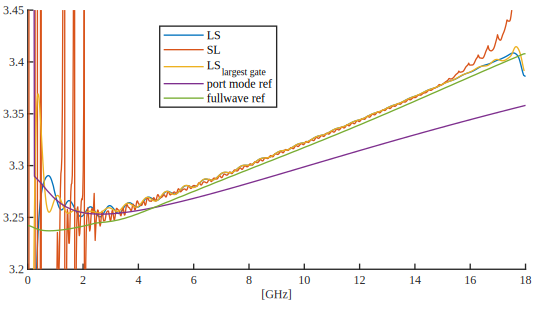
\includegraphics[width=\textwidth]{epsisim}
        \caption{Simulated data retrieved effective permittivity compared with $\varepsilon_{eff}$ calculated from
        the $S_{21}$ of a full--wave simulation of a microstrip section (terminated on adaptive waveguide ports),
            and effective dielectric constant computed by the port mode solver of CST.}
        \label{fig:epsilonsim}
    \end{figure}
    \begin{figure}[!h]
        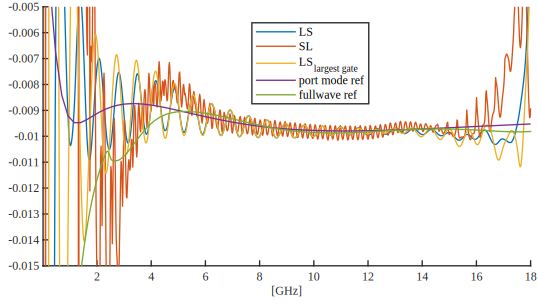
\includegraphics[width=\textwidth]{tandsim}
        \caption{Simulated data retrieved effective loss tangent compared with $\tan\delta_{eff}$ calculated from
        the $S_{21}$ of a full--wave simulation of a microstrip section (terminated on adaptive waveguide ports),
            and effective loss tangent computed by the port mode solver of CST.}
        \label{fig:tandsim}
    \end{figure}

    \subsection{Measurements}
    \label{subsec:measurements}
    \begin{figure}[!h]
        \includegraphics[width=\textwidth]{sparameas}
        \caption{De-embedding results from the measurements of the test fixtures.
        Solid lines: transmissivity (s), dotted lines: reflectivity (t);
        for all the reference fixture -- under test fixture combinations e.g. LS = long line as reference and short line de-embedding target.
        The transmissivity sign is chosen to always correspond to a negative-length section
        of lossy transmission line (for ease of comparison).}
        \label{fig:sparameas}
    \end{figure}

    \begin{figure}[!h]
        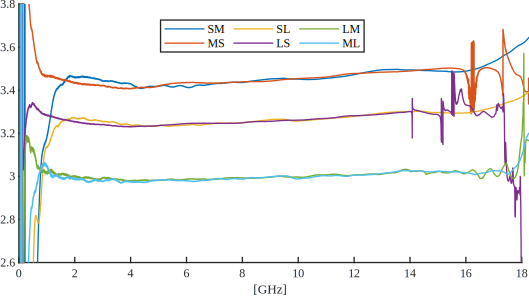
\includegraphics[width=\textwidth]{epsimeas}
        \caption{Measured data retrieved effective permittivity for all the reference fixture -- under test fixture combinations.}
        \label{fig:epsilonmeas}
    \end{figure}
    \begin{figure}[!h]
        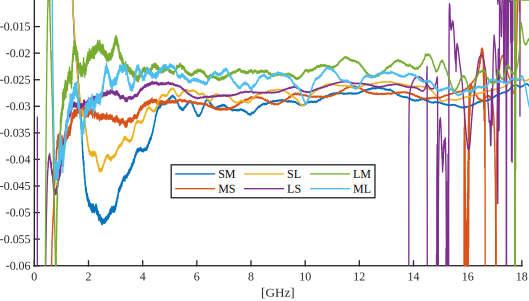
\includegraphics[width=\textwidth]{tandmeas}
        \caption{Measured data retrieved effective loss tangent for all the reference fixture -- under test fixture combinations.}
        \label{fig:tandmeas}
    \end{figure}


    \section{Non-identical fixtures de-embedding error}
    \label{sec:error}

    \subsection{Measurement results}
    \label{subsec:measure-error}


    \section{Numerical model matching}
    \label{sec:numerical-model-matching}


    \section{Conclusions}
    \label{sec:conclusion}


    \clearpage
    \bibliographystyle{IEEEtran}
    \bibliography{bibliography}

\end{document}

